% Name: Taylor polynomials
% Description: sin x and its Taylor polynomials of degree 1, 3, 5, and 7 about 0, each hugging the curve over a wider stretch than the last.
% Tags: Taylor polynomial, Taylor series, approximation, sine

\usetikzlibrary{arrows.meta}

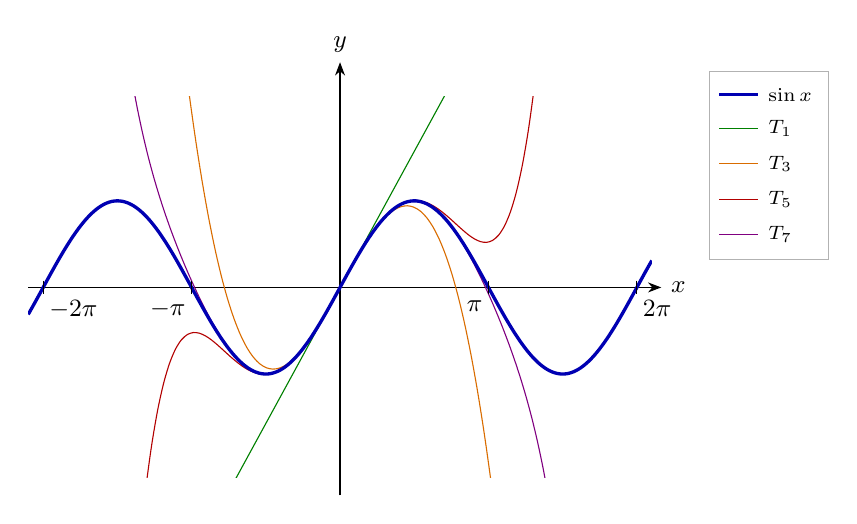
\begin{tikzpicture}[>={Stealth}, xscale=0.6, yscale=1.1, every node/.style={font=\small}]
  \draw[->] (-6.6,0) -- (6.8,0) node[right] {$x$};
  \draw[->] (0,-2.4) -- (0,2.6) node[above] {$y$};
  % Each polynomial in nested form, x(1 - x²/6(1 - x²/20(1 - x²/42))), so TeX's arithmetic never sees x⁷
  \begin{scope}
    \clip (-6.6,-2.2) rectangle (6.6,2.2);
    \draw[thin, green!50!black, domain=-3:3, samples=40] plot (\x, {\x});
    \draw[thin, orange!85!black, domain=-4:4, samples=60, smooth] plot (\x, {\x*(1 - \x*\x/6)});
    \draw[thin, red!70!black, domain=-5:5, samples=80, smooth] plot (\x, {\x*(1 - \x*\x/6*(1 - \x*\x/20))});
    \draw[thin, violet, domain=-6:6, samples=100, smooth] plot (\x, {\x*(1 - \x*\x/6*(1 - \x*\x/20*(1 - \x*\x/42)))});
    \draw[very thick, blue!70!black, domain=-6.6:6.6, samples=120, smooth] plot (\x, {sin(deg(\x))});
  \end{scope}
  % Each tick's label goes on the side where sin x is above the axis, clear of the curve
  \foreach \x/\l/\a in {-6.2832/-2\pi/north west, -3.1416/-\pi/north east, 3.1416/\pi/north east, 6.2832/2\pi/north west} \draw (\x,0.08) -- (\x,-0.08) node[anchor=\a, inner sep=2pt] {$\l$};
  \matrix[anchor=north west, draw=gray!60, fill=white, inner sep=3pt, row sep=1pt, nodes={font=\scriptsize, anchor=west}] at (7.8,2.5) {
    \draw[very thick, blue!70!black] (0,0) -- (0.5,0); & \node {$\sin x$}; \\
    \draw[thin, green!50!black] (0,0) -- (0.5,0); & \node {$T_1$}; \\
    \draw[thin, orange!85!black] (0,0) -- (0.5,0); & \node {$T_3$}; \\
    \draw[thin, red!70!black] (0,0) -- (0.5,0); & \node {$T_5$}; \\
    \draw[thin, violet] (0,0) -- (0.5,0); & \node {$T_7$}; \\
  };
\end{tikzpicture}
